\chapter{Practical examples}
\label{chapter3}

\noindent 
% remove: \citep{paper:pacs}

%---------------------------------------------------------------
\section{Application to particle-size curves in heterogeneous aquifers}
We consider here a data set, kindly provided by professor Menafoglio, obtained at the Lauswiesen site, located in the Neckar river valley, near the city of T\"{u}bingen (Germany). \\ 
The subsurface system in the area has been characterized through extensive information obtained at a number of boreholes, which are employed to perform sedimentological as well as hydraulic analyses.

Of specific relevance to our study are the available 406 particle-size curves (PSCs) sampled along 12 fully penetrating vertical boreholes.
Figure \ref{fig:boreholes} depicts a sketch of the borehole network and sampling locations at the site. 

\begin{figure}
	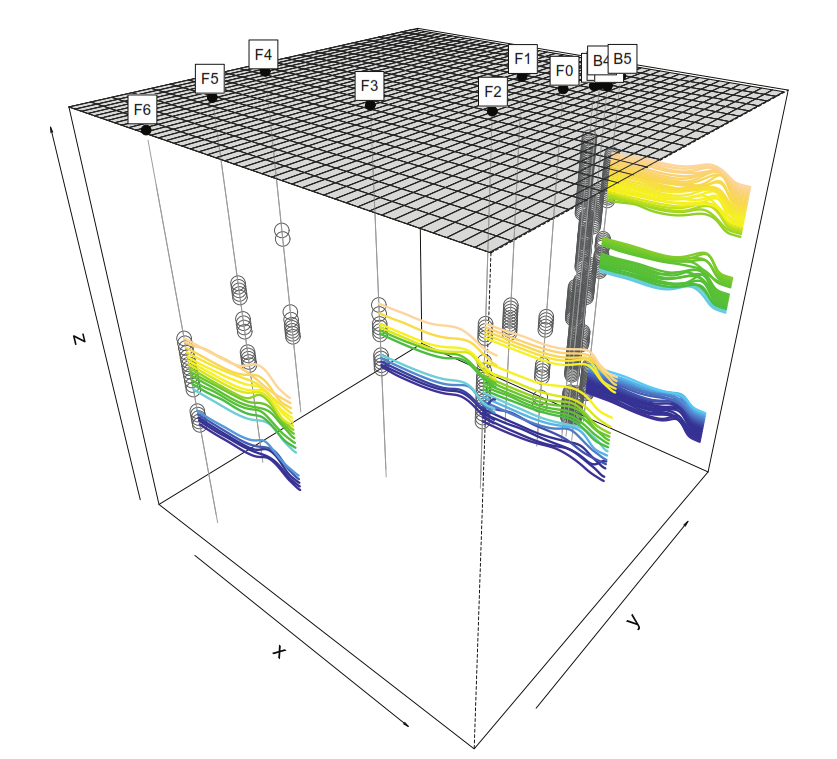
\includegraphics[width=8cm]{./pictures/psc/particle_size_densities.png}
	\centering
	\caption{Three-dimensional representation of particle-size densities at the Lauswiesen site. Grey points represent measurement locations, colored curves represent a subset of the dataset of PSCs. Colors indicate the depth of the sampling locations along the borehole.}
	\label{fig:boreholes}	
\end{figure}

The aquifer is made up by alluvial material overlain by stiff silty clay and underlain by hard silty clay. The site characterization has been based on stratigraphic information
collected at a set of monitoring and pumping wells.  \\
PSCs describe the local distributions of grain sizes within the aquifer system.
A set of twelve discrete sieve diameters (i.e., from a minimum of 0.063 up to 100.0 mm) were employed to reconstruct these curves by way of grain sieve analysis on soil samples, as in \ref{fig:sieve}.  

\begin{figure}
	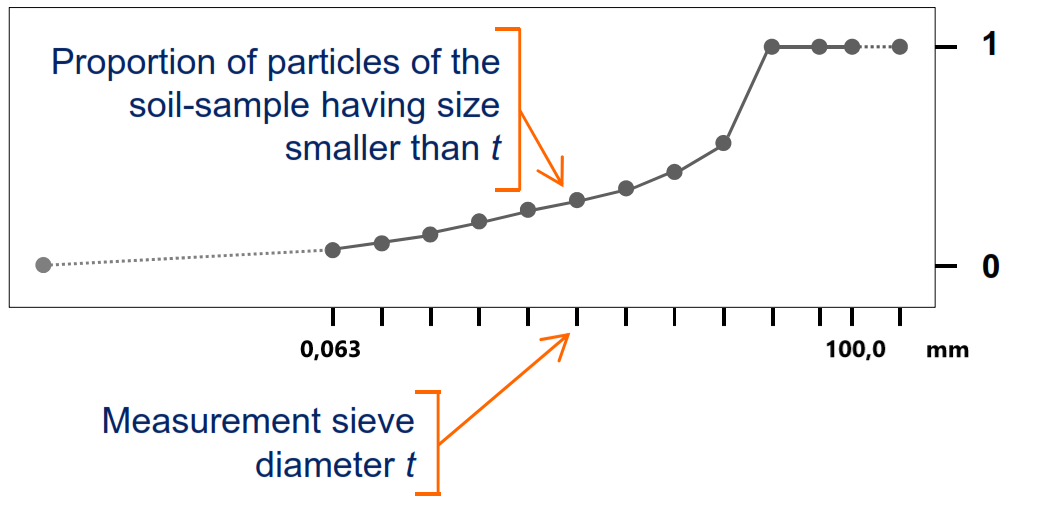
\includegraphics[height=3.5cm]{./pictures/psc/psc.png}
	\centering
	\caption{Example of particle-size raw data from sieze measurements, from clay and silt grains up to granules and pebbles.  \\
	We interpret PSCs as cumulative distribution functions and their derivatives as probability density functions. 
	Grain sieve analysis of soil samples, indeed, yields a discrete representation of the curves by measuring selected particle diameters which, in turn, correspond to quantiles of the particle-size curve.}
	\label{fig:sieve}	
\end{figure}

From the mathematical viewpoint, a particle-size density is a probability density function, associated with the distribution of particle sizes within a given soil sample. 

As such, available data consist of a set of constrained curves, spatially distributed. The statistical characterization of PSCs plays a key role in the classification of soil types, for inferring hydraulic parameters (e.g., porosity, permeability and hydraulic conductivity), and reconstructing the internal architecture of the groundwater system. 

In this vein, the study of PSCs may be concerned, as in \citep{menafoglio:psc}, with a geostatistical analysis, e.g. in order to identify clusters which represent the occurrence of different soil types and distinguish geomaterials at the site, and to characterize the spatial distribution of each identified textural class, and to provide Kriging estimates of the heterogeneous distribution of PSCs at unsampled locations. \\
Classification of aquifer geomaterials and estimation of their spatial arrangement is relevant to properly reconstruct the internal architecture of groundwater systems which can play a critical role in controlling contaminant spreading on different scales. 

As already pointed out, in the present case study an estimate of the particle-size curve at a given spatial location \textit{s} is available only for a set of \text{N} = 12 sieve diameters.  \\
To achieve any of the goals listed above, as in several other practical field situations, preprocessing of the raw data is required to obtain smooth estimates of the PSCs and associated densities.

The support of the PSCs has been assumed to be compact, upon setting the data support as \text{I} = $[\log(0.001),\log(200)]$, consistent with the type of lithology at the site.

Figure \ref{fig:psc_smoothed} depicts the resulting smoothed curves, obtained applying the algorithm described in chapter \ref{problem}.

\begin{figure}[ht]
	
	\begin{subfigure}{.5\textwidth}
		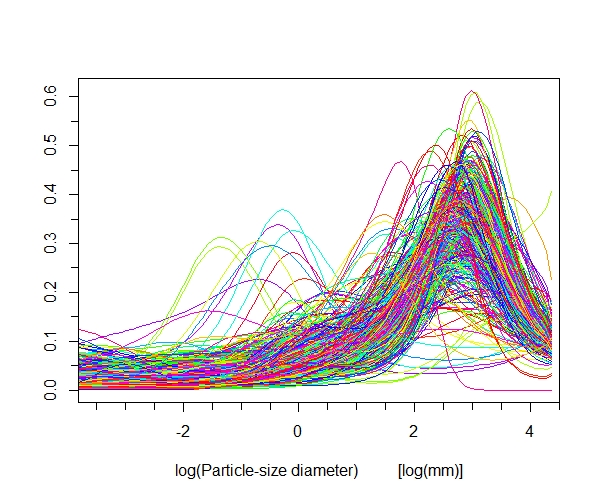
\includegraphics[width=6cm]{./pictures/psc/psc_all_res_4.jpeg} 
		\label{fig:subim1}
	\end{subfigure}
	\begin{subfigure}{.5\textwidth}
		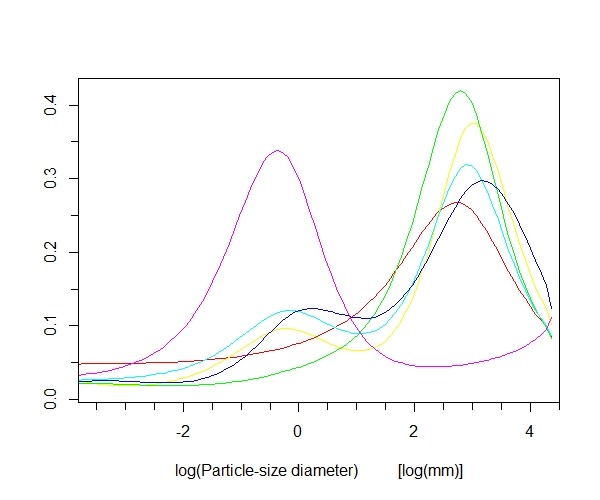
\includegraphics[width=6cm]{./pictures/psc/psc_few_res_4.jpeg}
		% \caption{Test C}
		\label{fig:subim2}
	\end{subfigure}
	
	\caption{Smoothed particle-size densities: on the left, all in one picture, and, on the rigth, just a few of them, chosen quite randomly, to highligth the variety in the soil composition for different sampling locations}
	\label{fig:psc_smoothed}
	
\end{figure}


%---------------------------------------------------------------
\section{Application to the well-known Iris flower data set}
The Iris flower data set is a multivariate data set introduced in the 1930s by Sir Ronald Fisher, who collected the data to quantify the morphologic variation of Iris flowers of three related species.
 
The dataset consists of 50 samples from each species of Iris flowers (Iris setosa, Iris virginica and Iris versicolor). Four features were measured from each sample, they are the length and the width of sepal and petal, in centimeters. 

We focus our attention on the variable related to the length of sepal, shown in figure \ref{fig:iris}.

\begin{figure}
	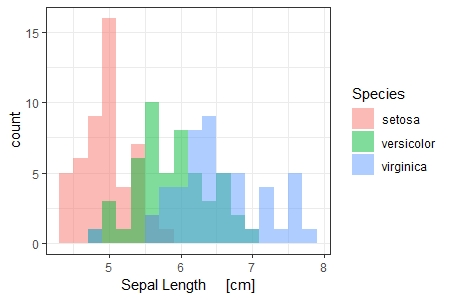
\includegraphics[height=3.5cm]{./pictures/iris/iris.jpeg}
	\centering
	\caption{Histogram of the variable Sepal Length for the Iris data set}
	\label{fig:iris}	
\end{figure}

The results are represented in figures \ref{fig:setosa} and \ref{fig:iris_v}: to be precise, the former shows how the algorithm works for different values of $\alpha$ when applied to the measures related to the Setosa species, the latter presents just the other two species for a fixed $\alpha$. 

It is worth remembering that the parameter $\alpha$ is related to the fidelity term - the higher it is, the more the output density is forced to stay near to the given values of the histogram.

\begin{figure}[ht]
	
	\begin{subfigure}{.5\textwidth}
		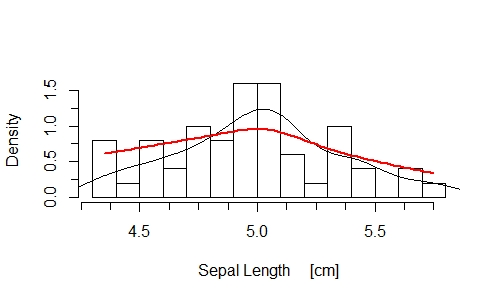
\includegraphics[width=6cm]{./pictures/iris/setosa_10.jpeg} 
		\caption*{$\alpha$ = 10}
		\label{fig:alpha10e1}
	\end{subfigure}
	\begin{subfigure}{.5\textwidth}
		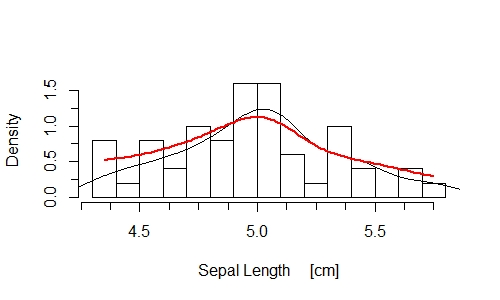
\includegraphics[width=6cm]{./pictures/iris/setosa_100.jpeg}
		\caption*{$\alpha$ = 100}
		\label{fig:alpha10e2}
	\end{subfigure}

	\begin{subfigure}{.5\textwidth}
		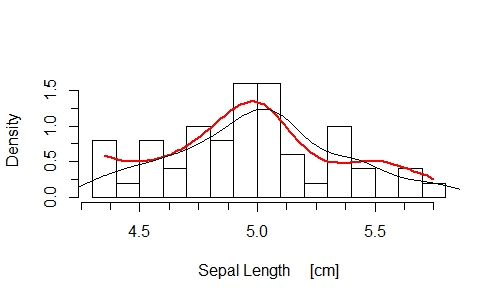
\includegraphics[width=6cm]{./pictures/iris/setosa_1000.jpeg} 
		\caption*{$\alpha$ = 1000}
		\label{fig:alpha10e3}
	\end{subfigure}
	\begin{subfigure}{.5\textwidth}
		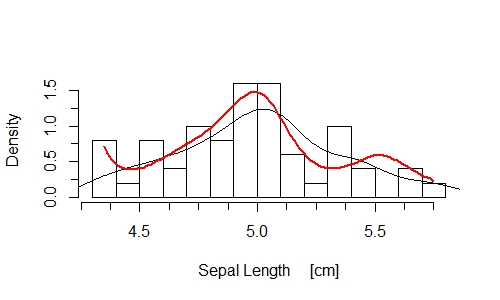
\includegraphics[width=6cm]{./pictures/iris/setosa_10000.jpeg}
		\caption*{$\alpha$ = 10000}
		\label{fig:alpha10e4}
	\end{subfigure}
	\caption{Data related to the Iris Setosa and the estimated density for different values of $\alpha$. The black line represents the "real" density, obtained from all the data through the kernel estimate. The coloured line is the density estimated with the algorithm - which is applied to the histograms.}
	\label{fig:setosa}
	
\end{figure}

\begin{figure}[ht]
	
	\begin{subfigure}{.5\textwidth}
		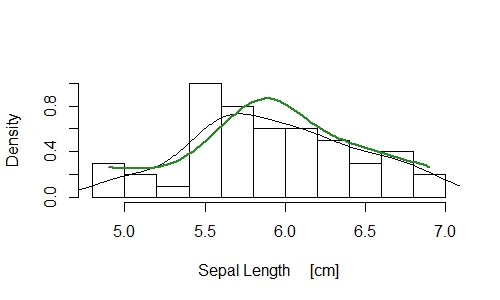
\includegraphics[width=6cm]{./pictures/iris/versicolor_100.jpeg} 
		\caption*{Iris Versicolor}
		\label{fig:versicolor}
	\end{subfigure}
	\begin{subfigure}{.5\textwidth}
		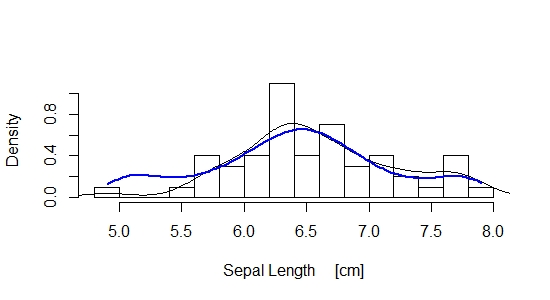
\includegraphics[width=6cm]{./pictures/iris/virginica_1000.jpeg}
		\caption*{Iris Virginica}
		\label{fig:virginica}
	\end{subfigure}
		
	\caption{Data related to the other two species of Iris. $\alpha$ is fixed and set to 1000.}
	\label{fig:iris_v}
	
\end{figure}




%---------------------------------------------------------------




